Besides stock prices, financial news can also be used as a proxy for business relationship. If an announcement was made or any relevant information like a SEC filing was released by a company, financial news report it as fast as possible. Longer reports put it even into a bigger picture, provide some background information and refer to possible competitors. Two companies are most likely mentioned together in the same article, if they are related to each other in any context. The simultaneous mentioning of two companies within one article is called co-occurrence in the following.

\subsection{Named Entity Recognition}

Before collecting co-occurrences, first the occurrence of each company needs to be extracted and linked separately. If an author is writing news, there are many problems for determining whether, and if so which, companies are the topical subject. He might use an alias name, a product of the company (e.g. \emph{Google} instead of \emph{Alphabet}) or just a representative like the CEO (e.g. \emph{Steve Jobs} instead of \emph{Apple}). As a first heuristic approach, only the occurrences of company names are considered. After applying NER on the corpus of financial news \footnote{Implementation by SpaCy: https://spacy.io}, all entities which are labeled as organizations like companies, agencies or institutions are collected. This results in 9.6 out of 40.7 million entities.

%  \todo{mention example (use elasticsearch)}
% \todo{Example snippet of news with different tagged organizations (and other tags}
% https://spacy.io/api/annotation#named-entities

% This requires to recognize corporation names which might be tackled using Named Entity Recognition (NER) or even more complex approaches as the algorithms by Rau \cite{Rau1991:extractNames} or Loster et al. \cite{Loster2017:comp_rec}.

\begin{figure}
    \centering
    \frame{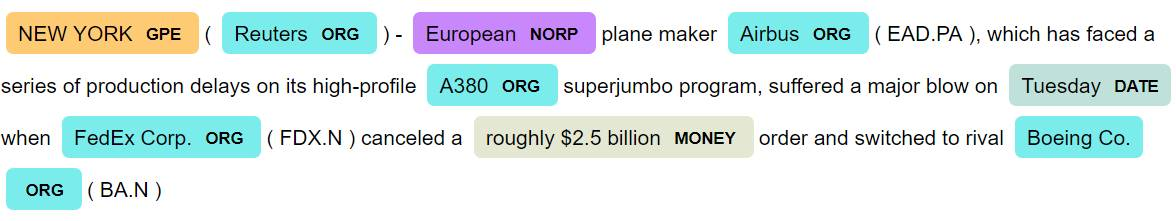
\includegraphics[width=\textwidth]{figures/text/entities-displacy.jpg}}
    \caption{Classified entities for the Reuters article \enquote{FedEx cancels Airbus A380 order, switches to Boeing} (2006-11-07). Each of the five entity types is marked by another color whereas organization are lightblue. An abbreviation of each label is added behind the labeled sequence in bold letters. For example, NORP represents nationalities among others and ORG represents companies, institutions, etc. The content reports a policy change by \emph{FedEx Corporation} in favour of \emph{Boeing Company}.} 
    \label{fig:ner-entities}
\end{figure}

To give an example, how a financial news article and extracted entities might look like, Figure~\ref{fig:ner-entities} shows a selected section in a Reuters article from the 7th of November, 2006. Although, the aircraft \emph{A380} is falsely recognized as an organization, the four mentioned companies are correctly tagged. One might note that in this example, stock symbols are already provided in brackets within the text. Even though, they can be used to set up a link between company and stock price, such additional information are often missing in the examined text-corpus. How these tagged organizations are automatically linked to companies on the stock market and thereby to the regarding stock prices, will be shown in the next section.


\subsection{Named Entity Linking}

Out of all organization entities, only those are of interest which can be linked to a company from the S\&P~500 market index. The official company name is provided by the stock dataset and linked to the correct stock prices by its stock symbol. The names contain unhandy suffixes like \emph{Inc.} or \emph{Limited} which are usually left out in the news. To establish the link between occurrences in news and the full corporate name, a regular expression is used to remove the name extensions from both values:

\DefineShortVerb{\!}
\SaveVerb{VerbA}! ,?[^\w](Corp\ A|A\ Corp|\&\ Co|Svc\.Gp| !
\SaveVerb{VerbB}! Corp(?:oration|'s)?|Inc|Co(?:s|mpany)?| !
\SaveVerb{VerbC}! Ltd|Limited|Plc|Group|(?:International| !
\SaveVerb{VerbD}! Int'l)(?:\ Inc)?|Int'l\ Industries)\.?$ !

\begin{align}
  \begin{split}
    \UseVerb{VerbA} \\ \UseVerb{VerbB} \\ \UseVerb{VerbC} \\ \UseVerb{VerbD}
  \end{split}
  \label{formula:linking_regex}  \\ \eqname{Regular Expression}
\end{align}

% After the suffices are removed from both sides, the remaining strings are not safely matching. To allow small deviations a fuzzy matching metric, namely the Damerau–Levenshtein distance \cite{Damerau1964}, is applied. It measures the edit distance between two strings considering the insertion, deletion, substitution and transposition of characters.

If the regular expression reduced both strings to their least common sequence and they are completely equal, the extracted entity is assumed to match the examined stock company. In the end, 436.000 related company names were extracted which are distributed over 127.000 articles. Because occurrences were only found for 443 companies, the remaining companies are removed in the remainder of this study.

\begin{figure}
    \centering
    \frame{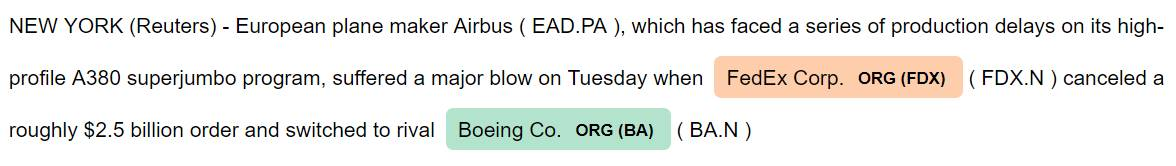
\includegraphics[width=\textwidth]{figures/text/entities-displacy-org.jpg}}
    \caption{Linked companies for the same article as in Figure~\ref{fig:ner-entities}. Hereby, the colors are differing for each linked company. To indicate the established link, the bold tag behind the labeled sequence contains the regarding stock symbol.}
    \label{fig:ner-entities-org}
\end{figure}

Figure~\ref{fig:ner-entities-org} shows the same financial news article as before but highlights occurrences of linked company only. Two of four companies are linked to stock prices, whereas the remaining two are not considered since they are not components of the market index and thereby not contained by the data covered in this work.

\subsection{Co-occurrence Features}

To measure the relationship between two companies based on these occurrences, a feature needs to be found. Therefore, three different approaches are proposed:
% \begin{enumerate*}[label=(\roman*)]
%     \item Co-occurrences;
%     \item Minimum Distance;
%     \item Pairwise Distance
% \end{enumerate*}.
% https://arxiv.org/pdf/1506.07220.pdf

\begin{enumerate}[
leftmargin=0pt, itemindent=20pt,
labelwidth=15pt, labelsep=5pt, listparindent=0.7cm,
align=left, label={\textbf{(\arabic*)}}]
\item \textbf{Co-occurrences} of two companies is calculated by the number of articles in which both company names occur. If this is the case, the article is likely to write something about their business relationship. This feature does not account for the number or distance of occurrences for one company within one article. It rather measures the co-occurrences across the whole text corpus instead of weighting the connection within one article.
\item \textbf{Minimum Distance} takes the intra-article connection into account by calculating the distance for each possible pair of company names within one article. Subsequently, the smallest possible distance is kept for this article. The distance between two entities is represented by the starting indices of the initially matched string. To unite the article-wise values, all minimum distances across all articles are averaged. If two companies are strongly connected, authors are more likely to provide comparisons between them. This will be reflected by an average smaller distance for co-occurrences of two companies across all articles.
\item \textbf{Pairwise Distance} is a more sophisticated approach compared to the previous ones. It accounts for the multiple inter-article co-occurrences as well as the multiple intra-article co-occurrences. Therefore, a scan line algorithm will traverse all occurrences of these two companies in an article and pair these up while avoiding a too high distance. Similar to the previous approach, all distances are averaged but, in addition, each pair is considered instead of only considering the best one for each article.
\end{enumerate}

For these three features the suitability will be evaluated in the next section when they are compared to the previously generated stock price correlations. To provide a first examination of text-based features in general, a graph is shown in Figure~\ref{fig:graph-cooccurrence-pairwise} which was generated in the same fashion as previously done for the cross-correlations among prewhitened stock prices. The strength of edges is calculated by their pairwise distance across the whole news corpus. Because there are 15.184 pairs with a non-zero pairwise distance, all values below the 99.9th percentile are left out. This resulted in 90 edges between 98 nodes from all eleven industry sectors. As already stated in respect to the previous graph, the graph consists of the most extreme values and therefore is not a representative sample for the entire graph.

% 0.994, 0.4985 with people and halved

\begin{figure}
    \centering
    \begin{subfigure}[b]{\textwidth}
        \centering
        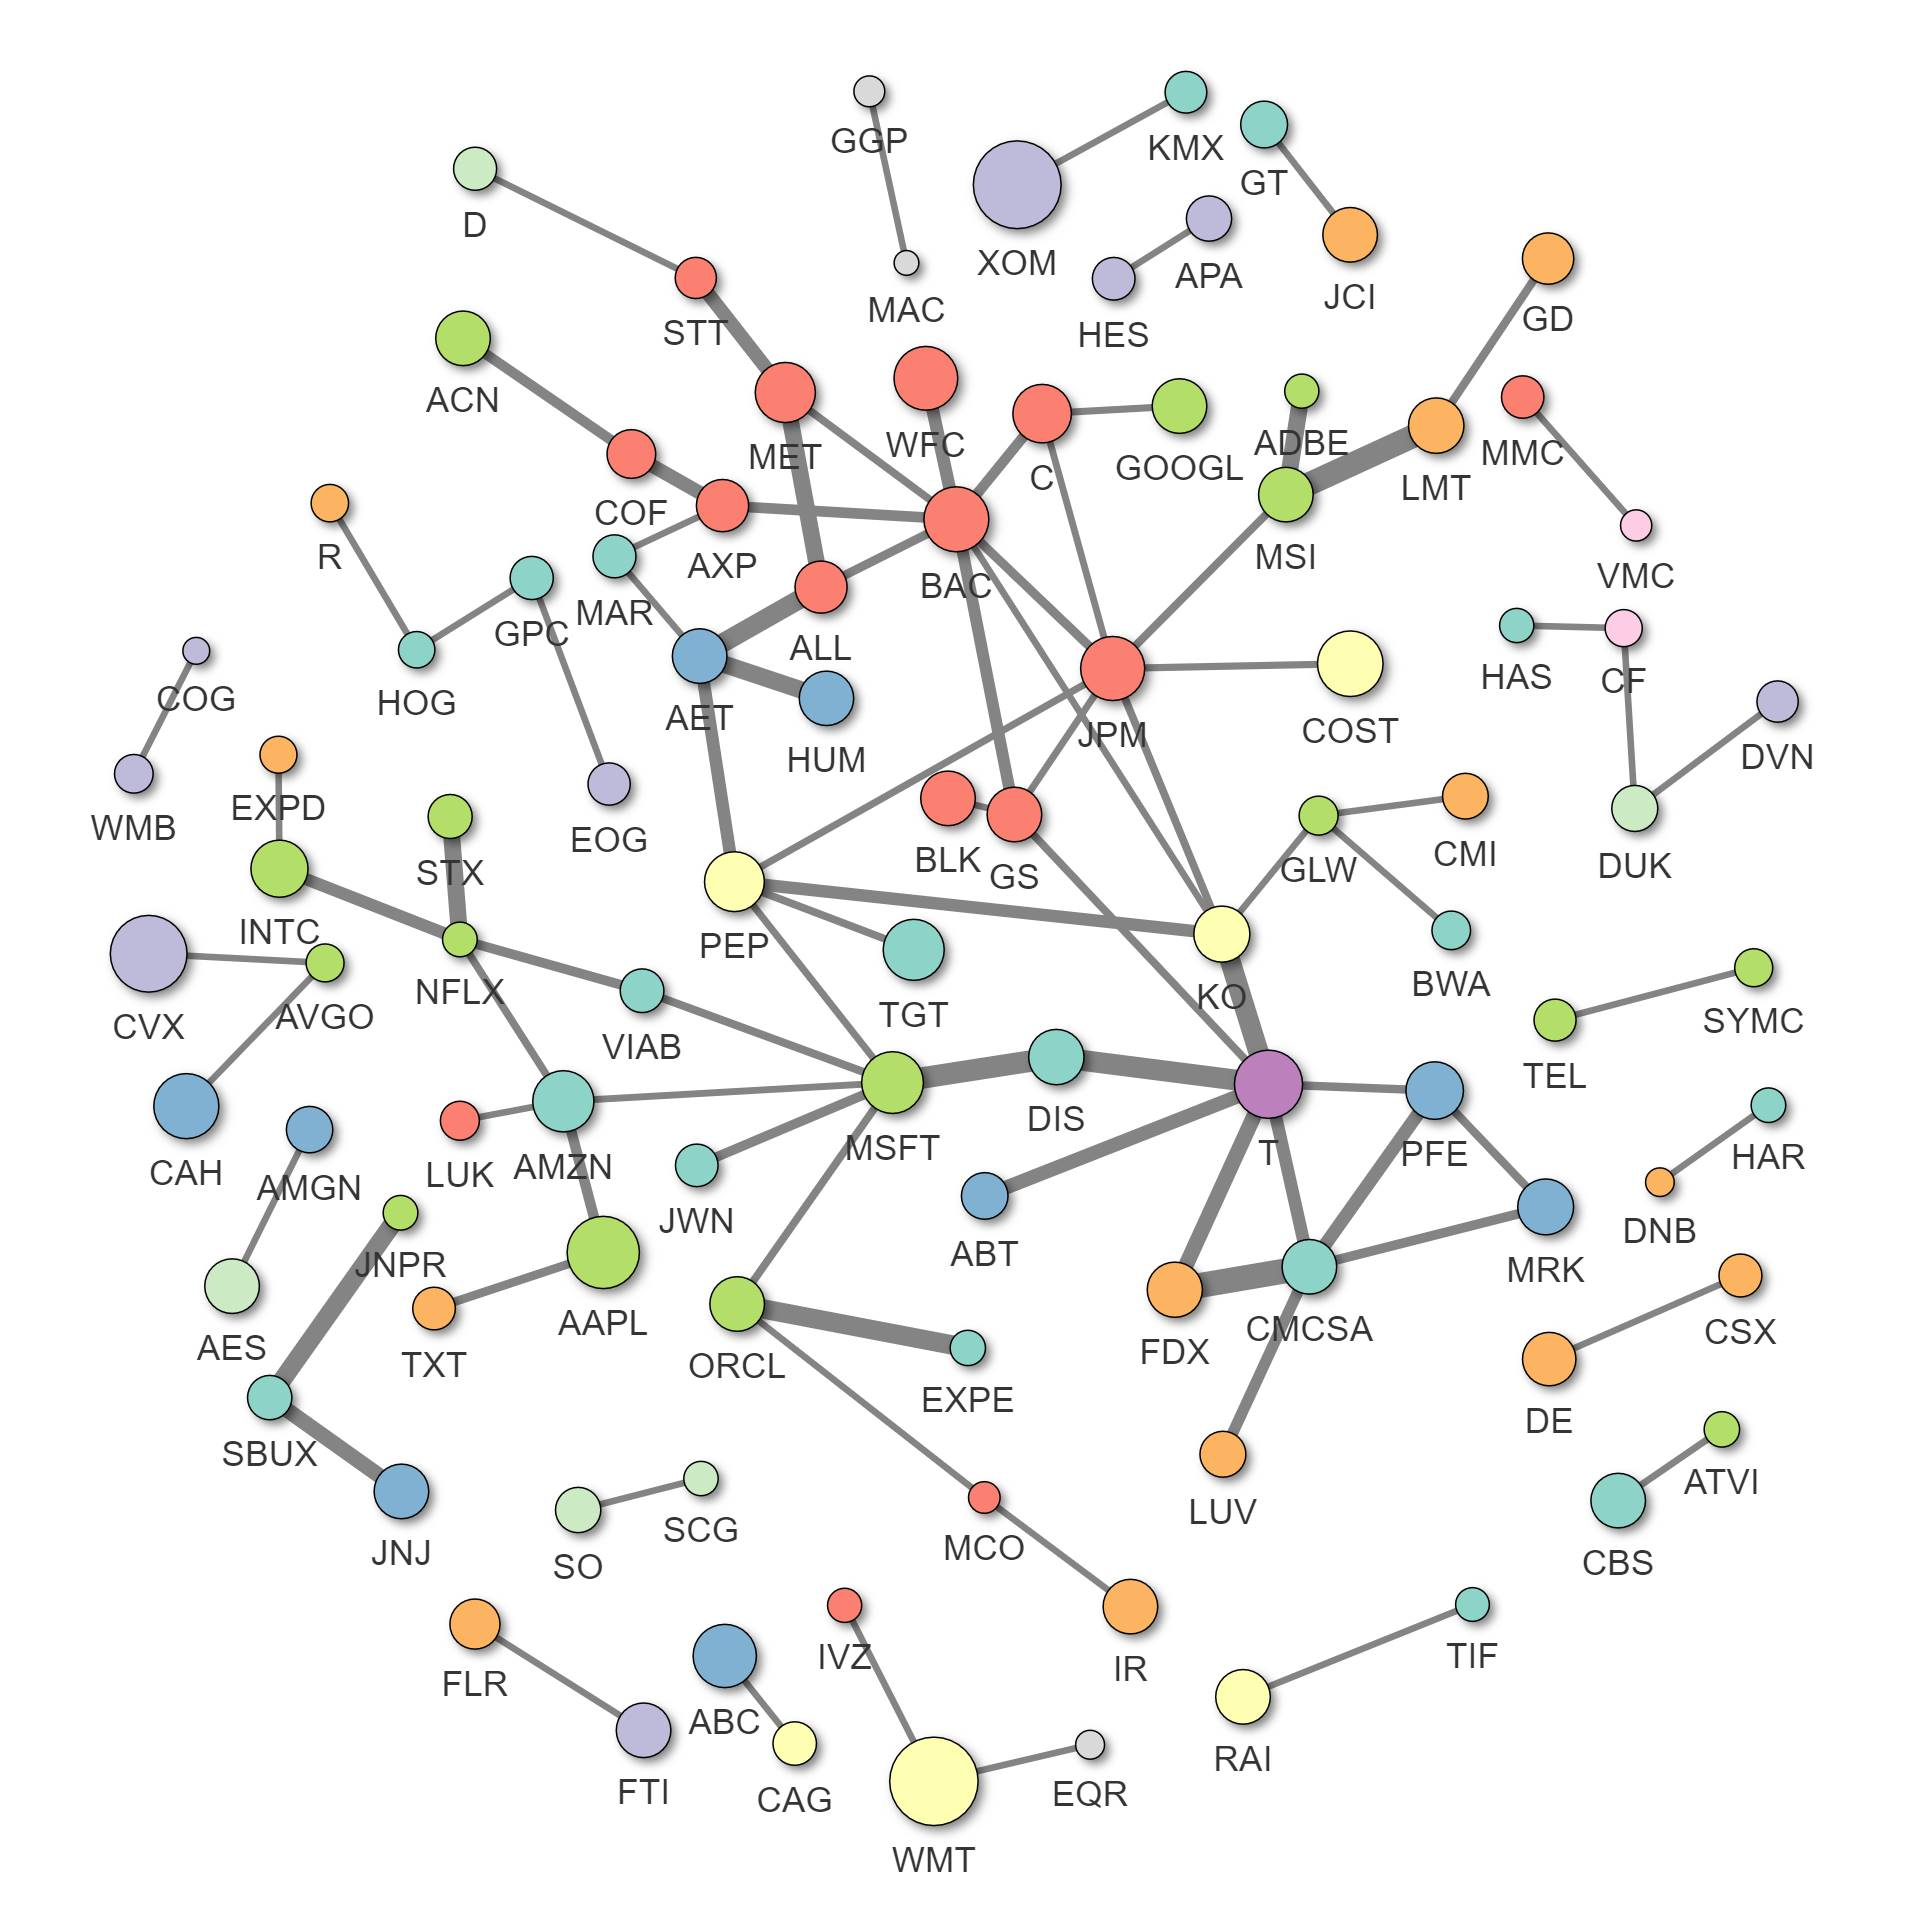
\includegraphics[width=\textwidth]{figures/text/graph-pair-dist-999-42.jpg}
    \end{subfigure}
    \vfill
    \begin{subfigure}[b]{\textwidth}
        \centering
        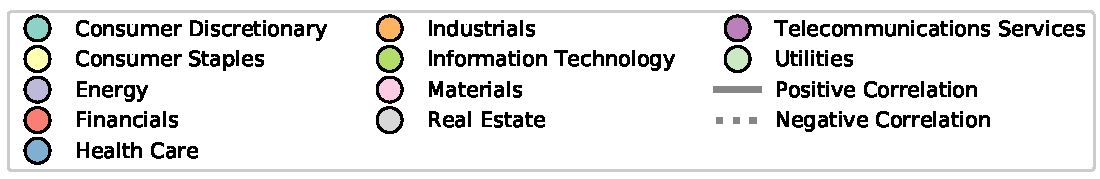
\includegraphics[width=\textwidth]{figures/graph-legend.pdf}
    \end{subfigure}

    \caption{Graph of the 90 strongest connections, measured by the calculated pairwise distance among two companies. Each node represents one company which is labeled by the companies ticker symbol and coloured by the regarding industry section. Which color belongs to which industry is provided by the legend below. The node's size is determined by the total revenue for this company. Each edge between two nodes represents the pairwise distance between the co-occurrences of the regarding companies. More extreme values are indicated by a thicker edge.}
    \label{fig:graph-cooccurrence-pairwise}
\end{figure}

Compared to the correlation graph in Figure~\ref{fig:graph-correlations}, this one reveals a very different structure. Both graphs share 29 nodes and four edges only. Instead of many small decoupled subgraphs for industry sectors this graph reveals one big subgraph consisting of 50 nodes from many different industry sectors. Some edges between companies sound comprehensible after investigating their business relationships. For example, \emph{Microsoft Corp.} (\emph{MSFT}) and \emph{Viacom Inc.} announced a long-term strategic alliance for corporate segments like game development and advertisement in 2007. To mention another example, a high pairwise distance can be observed for both streaming providers \emph{Netflix Inc.} (\emph{NFLX}) and \emph{Amazon.com Inc.} (\emph{AMZN}) which both benefit from the increased demand in this segment of the market.

Over the whole graph, only 28 edges are connections among companies originating from the same industry. The greatest industry cluster can be observed for companies from the sector \emph{Financials} which includes insurance companies (e.g. \emph{American International Group, Inc.}), investment banks (e.g. \emph{JPMorgan Chase \& Co.}) and financial service providers (e.g. \emph{Citigroup Inc.}). Some of them are densely connected with other industries which can be argued by their investments in stocks of other companies.


% No stock prices between 2006 and 2010. Check if the features extracted from this span is relevant.

% Word Embedding Distance
% General Embedding
% Domain-based

% Co-Mentioning Network from News text: https://link.springer.com/chapter/10.1007/978-3-319-92871-5_7


% Prediction
% Averaged Word Vectors vs. Tfidf Vectors	
% Most common words during up/down
% Sentiment vs Price Movement
%   For further analyses drop all entities from text

% \missingfigure[figwidth=6cm]{Testing a long text string}